\subsection{Memory Models with Relaxed Ordering}

The following models are \textbf{grouped based on the types of memory operation reordering} they allow. Each model applies the relaxing memory models, so they allow certain memory operation orders to be violated to improve performance.

\highspace
Before introducing each memory model, we will talk about problems and possible solutions for memory models with relaxed order.

\highspace
\begin{flushleft}
    \textcolor{Red2}{\faIcon{exclamation-triangle} \textbf{Problems with Memory Reordering}}
\end{flushleft}
Reordering of memory operations can lead to \textbf{inconsistencies} and \textbf{unpredictable behavior} in multiprocessor systems.

\highspace
\begin{flushleft}
    \textcolor{Green3}{\faIcon{check-circle} \textbf{Solutions: Synchronization Primitives}}
\end{flushleft}
\begin{itemize}
    \item[\textcolor{Green3}{\faIcon{check}}] \textcolor{Green3}{\textbf{Memory Fence Instructions (Barriers)}}: \textbf{Prevent reorderings by ensuring that all memory operations before the fence complete before any new operations begin}.
    
    Fence instructions can be costly in terms of performance but are essential for maintaining order and consistency.


    \item[\textcolor{Green3}{\faIcon{check}}] \textcolor{Green3}{\textbf{Read-Modify-Write}}: Ensures atomic read and write operations to a memory location.


    \item[\textcolor{Green3}{\faIcon{check}}] \textcolor{Green3}{\textbf{Compare-and-Swap}}: Atomically compares a memory location's value and swaps it if it matches a specified value.


    \item[\textcolor{Green3}{\faIcon{check}}] \textcolor{Green3}{\textbf{Transactional Memory}}: Allows a group of memory operations to be executed atomically.
\end{itemize}

\newpage

\subsubsection{Allowing Reads to Move Ahead of Writes}

\begin{flushleft}
    \textcolor{Green3}{\faIcon{question-circle} \textbf{Which memory operation is relaxed?}}
\end{flushleft}
Given the four memory operation sequences (see detailed explanation on page \hqpageref{flushleft: Memory Operation Ordering}), the relaxed operations are marked as cancel:
\begin{itemize}
    \item[\textcolor{Green3}{\faIcon{check}}] \textcolor{Green3}{\textbf{\emph{Relaxed}} $\cancel{W_{X} \rightarrow R_{Y}}$}: \textbf{Write to $X$ must commit before a subsequent read from $Y$}.

    This means that if a write to memory location $X$ occurs before a read from another memory location $Y$ in the program order, the write must be complete and visible before the read.


    \item[\textcolor{Red2}{\faIcon{times}}] \important{$R_{X} \rightarrow R_{Y}$}: Read from $X$ must commit before a subsequent read from $Y$.
    \item[\textcolor{Red2}{\faIcon{times}}] \important{$R_{X} \rightarrow W_{Y}$}: Read from $X$ must commit before a subsequent write to $Y$.
    \item[\textcolor{Red2}{\faIcon{times}}] \important{$W_{X} \rightarrow W_{Y}$}: Write to $X$ must commit before a subsequent write to $Y$.
\end{itemize}
\begin{figure}[!htp]
    \centering
    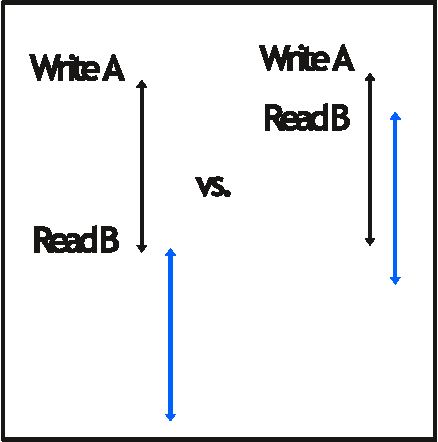
\includegraphics[width=.4\textwidth]{img/tso-and-pc-1.pdf}
\end{figure}

\newpage

\begin{flushleft}
    \textcolor{Green3}{\faIcon{book} \textbf{Models}}
\end{flushleft}
\begin{itemize}
    \item \hqlabel{definition: Total Store Ordering (TSO)}{\definition{Total Store Ordering (TSO)}}
    \begin{flushleft}
        \textcolor{Green3}{\faIcon{tools} \textbf{How does it work?}}
    \end{flushleft}
    It allows a processor to read a variable (e.g., \texttt{B}) before its write to another variable (e.g., \texttt{A}) is visible to all processors ($\cancel{W_{\texttt{A}} \rightarrow R_{\texttt{B}}}$).

    This enables the processor to hide the latency of write operations by \textbf{allowing reads to proceed independently}.

    \begin{flushleft}
        \textcolor{Red2}{\faIcon{exclamation-triangle} \textbf{Implications}}
    \end{flushleft}
    Other processors cannot see the new value of \texttt{A} (the value written to register \texttt{A}) until the write to \texttt{A} is observed by all processors.

    Only $W_{\texttt{A}} \rightarrow R_{\texttt{B}}$ order is relaxed, while $W_{\texttt{A}} \rightarrow W_{\texttt{B}}$ constraints still exist, meaning writes by the same thread occur in program order. Other processors see these writes in the correct order, but there might be a delay before the writes are visible due to buffering.

    \item \hqlabel{definition: Processor Consistency (PC)}{\definition{Processor Consistency (PC)}}
    \begin{flushleft}
        \textcolor{Green3}{\faIcon{tools} \textbf{How does it work?}}
    \end{flushleft}
    Similar to TSO, but with slightly \textbf{more flexibility}.

    Any processor can read the new value of \texttt{A} \textbf{before the write is observed by all processors}, allowing reads to be even \textbf{more independent} of writes.

    \begin{flushleft}
        \textcolor{Red2}{\faIcon{exclamation-triangle} \textbf{Implications}}
    \end{flushleft}
    Like TSO, only $W_{\texttt{A}} \rightarrow R_{\texttt{B}}$ order is relaxed, and $W_{\texttt{A}} \rightarrow W_{\texttt{B}}$ constraints remain, ensuring that writes by the same thread occur in program order.
\end{itemize}

\highspace
\begin{flushleft}
    \textcolor{Green3}{\faIcon{balance-scale} \textbf{Main differences between TSO and PC}}
\end{flushleft}
\begin{enumerate}
    \item \important{Read Flexibility}
    \begin{itemize}
        \item \textbf{TSO}: Reads by a processor can move ahead of its own writes.
        \item \textbf{PC}: Reads by any processor can observe new values of writes \textbf{\emph{before they are globally visible}}, allowing even more flexibility.
    \end{itemize}

    \item \important{Write Order}
    \begin{itemize}
        \item \textbf{Both Models}: Maintain the order of writes within the same processor, ensuring that $W_{\texttt{A}} \rightarrow W_{\texttt{B}}$ order is preserved.
    \end{itemize}

    \item \important{Performance vs. Complexity}
    \begin{itemize}
        \item \textbf{TSO}: Strikes a \textbf{\emph{balance between performance and simplicity}} by allowing limited reordering of reads and writes.
        \item \textbf{PC}: Offers \emph{\textbf{greater flexibility in read operations}}, potentially improving performance but at the \textbf{\emph{cost of slightly increased complexity}}.
    \end{itemize}
\end{enumerate}

\newpage

\subsubsection{Allowing writes to be reordered}

\begin{flushleft}
    \textcolor{Green3}{\faIcon{question-circle} \textbf{Which memory operation is relaxed?}}
\end{flushleft}
Given the four memory operation sequences (see detailed explanation on page \hqpageref{flushleft: Memory Operation Ordering}), the relaxed operations are marked as cancel:
\begin{itemize}
    \item[\textcolor{Green3}{\faIcon{check}}] \textcolor{Green3}{\textbf{\emph{Relaxed}} $\cancel{W_{X} \rightarrow R_{Y}}$}: \textbf{Write to $X$ must commit before a subsequent read from $Y$}.

    This means that if a write to memory location $X$ occurs before a read from another memory location $Y$ in the program order, the write must be complete and visible before the read.


    \item[\textcolor{Red2}{\faIcon{times}}] \important{$R_{X} \rightarrow R_{Y}$}: Read from $X$ must commit before a subsequent read from $Y$.
    \item[\textcolor{Red2}{\faIcon{times}}] \important{$R_{X} \rightarrow W_{Y}$}: Read from $X$ must commit before a subsequent write to $Y$.
    \item[\textcolor{Green3}{\faIcon{check}}] \textcolor{Green3}{\textbf{\emph{Relaxed}} $\cancel{W_{X} \rightarrow W_{Y}}$}: \textbf{Write to $X$ must commit before a subsequent write to $Y$}.

    This ordering ensures that if a write to $X$ happens before a write to $Y$ in the program, the first write must be completed before the second write is performed.
\end{itemize}

\highspace
\begin{flushleft}
    \textcolor{Green3}{\faIcon{book} \textbf{Models}}
\end{flushleft}
\begin{itemize}
    \item \definition{Partial Store Ordering (PSO)}
    \begin{flushleft}
        \textcolor{Green3}{\faIcon{tools} \textbf{How does it work?}}
    \end{flushleft}
    PSO allows more \textbf{aggressive reordering of write operations} compared to TSO (page \hqpageref{definition: Total Store Ordering (TSO)}) and PC (page \hqpageref{definition: Processor Consistency (PC)}).

    \begin{flushleft}
        \textcolor{Red2}{\faIcon{exclamation-triangle} \textbf{Implications}}
    \end{flushleft}
    \begin{itemize}
        \item Thread 1 on Processor 1 (\texttt{P1})
        \begin{lstlisting}
A = 1;
flag = 1;\end{lstlisting}

        \item Thread 2 on Processor 2 (\texttt{P2})
        \begin{lstlisting}
while (flag == 0); 
print A;\end{lstlisting}
    \end{itemize}

    \texttt{P2} may observe the change to \texttt{flag} before the change to \texttt{A}. This shows that PSO allows writes to \texttt{A} and \texttt{flag} to be reordered, improving write performance but potentially complicating program reasoning.

    \newpage

    \begin{flushleft}
        \textcolor{Green3}{\faIcon{check-circle} \textbf{Benefits}}
    \end{flushleft}
    \begin{itemize}
        \item $W_{X} \rightarrow W_{Y}$. \textcolor{Green3}{\textbf{Write Buffering}}: \textbf{Processors can reorder write operations in a write buffer}. For example, one write might be a cache miss while another is a cache hit, and reordering them can optimize performance.
        
        \item  $R_{X} \rightarrow R_{Y}$, $R_{X} \rightarrow W_{Y}$. \textcolor{Green3}{\textbf{Instruction Reordering}}: \textbf{Processors can reorder independent read and write instructions within the instruction stream}, leveraging out-of-order execution to maximize efficiency.
    \end{itemize}
    These reorderings and optimizations are particularly \textbf{effective in single instruction streams}, where dependencies between instructions are well understood and managed.
\end{itemize}

\newpage

\subsubsection{Allowing all reorderings}

\begin{flushleft}
    \textcolor{Green3}{\faIcon{question-circle} \textbf{Which memory operation is relaxed?}}
\end{flushleft}
Given the four memory operation sequences (see detailed explanation on page \hqpageref{flushleft: Memory Operation Ordering}), the relaxed operations are marked as cancel:
\begin{itemize}
    \item[\textcolor{Green3}{\faIcon{check}}] \textcolor{Green3}{\textbf{\emph{Relaxed}} $\cancel{W_{X} \rightarrow R_{Y}}$}: \textbf{Write to $X$ must commit before a subsequent read from $Y$}.

    This means that if a write to memory location $X$ occurs before a read from another memory location $Y$ in the program order, the write must be complete and visible before the read.


    \item[\textcolor{Green3}{\faIcon{check}}] \textcolor{Green3}{\textbf{\emph{Relaxed}} $\cancel{R_{X} \rightarrow R_{Y}}$}: \textbf{Read from $X$ must commit before a subsequent read from $Y$}.

    This order ensures that if a read from $X$ occurs before a read from $Y$ in the program, the first read must be completed before the second read occurs.


    \item[\textcolor{Green3}{\faIcon{check}}] \textcolor{Green3}{\textbf{\emph{Relaxed}} $\cancel{R_{X} \rightarrow W_{Y}}$}: \textbf{Read from $X$ must commit before a subsequent write to $Y$}.

    This means that if a read from $X$ occurs before a write to $Y$ in the program order, the read must be completed before the write is performed.


    \item[\textcolor{Green3}{\faIcon{check}}] \textcolor{Green3}{\textbf{\emph{Relaxed}} $\cancel{W_{X} \rightarrow W_{Y}}$}: \textbf{Write to $X$ must commit before a subsequent write to $Y$}.

    This ordering ensures that if a write to $X$ happens before a write to $Y$ in the program, the first write must be completed before the second write is performed.
\end{itemize}

\highspace
\begin{flushleft}
    \textcolor{Green3}{\faIcon{book} \textbf{Models}}
\end{flushleft}
\begin{itemize}
    \item \definition{Weak Ordering (WO)}
    \begin{flushleft}
        \textcolor{Green3}{\faIcon{tools} \textbf{How does it work?}}
    \end{flushleft}
    Operations are divided into critical and non-critical sections. Reordering is allowed outside of critical sections to maximize performance.

    \example{Example}: Can reorder any non-critical operations to enhance efficiency, executing them independently.


    \item \definition{Release Consistency (RC)}
    \begin{flushleft}
        \textcolor{Green3}{\faIcon{tools} \textbf{How does it work?}}
    \end{flushleft}
    Divides operations into acquire and release categories, allowing extensive reordering within these categories.

    \example{Example}: Reorders operations within acquire or release phases, enabling significant performance gains.
\end{itemize}
In these models, there are \textbf{no strict guarantees about the order of operations on data}. Essentially, everything can be reordered.

\begin{flushleft}
    \textcolor{Green3}{\faIcon{question-circle} \textbf{Why allow all reorders?}}
\end{flushleft}
By overlapping multiple reads and writes, the \textbf{system can execute reads as early as possible and delay writes as late as possible}, effectively \textbf{hiding memory latency} and \textbf{increasing performance}.